% Final report for ARIN 5203.
\documentclass[10pt,twocolumn,letterpaper]{article}

\usepackage[pagenumbers]{cvpr}
\usepackage{graphicx}
\usepackage{amsmath}
\usepackage{amssymb}
\usepackage{booktabs}
\usepackage{hyperref}

\def\cvprPaperID{ARIN5203}
\def\confName{ARIN 5203}
\def\confYear{2026}

\begin{document}

\title{Fine-Grained Bird Recognition with Annotated Foreground Regions}

\author{Zheng Shisheng\\
The Hong Kong University of Science and Technology\\
{\tt\small 21332987}
\and
Lu Yang\\
The Hong Kong University of Science and Technology\\
{\tt\small 21329126}
}

\maketitle

\begin{abstract}
We study how foreground localization, geometric preprocessing, and training
strategy affect fine-grained bird recognition on CUB-200-2011. Using an
ImageNet-pretrained ResNet-18 and a fixed class-stratified validation split,
we compare whole-image inputs, annotated bird boxes processed with center
cropping, and bird boxes processed with aspect-ratio-preserving letterboxing.
We then isolate the effect of the bird box with a matched whole-image
letterbox control, compare frozen and fine-tuned backbones, and ablate the
amount of context retained around the bird. The selected model uses the exact
annotated bird box, letterboxing, and full fine-tuning from the first epoch.
Across three training seeds it reaches $76.06\%\pm1.54\%$ validation Top-1.
The selected seed-43 checkpoint reaches $77.87\%$ Top-1, $94.15\%$ Top-5, and
$77.85\%$ Macro-F1 on the official 5,794-image test partition, compared with
$77.83\%$ validation Top-1. A background-only diagnostic collapses to
$1.61\%$ Top-1, whereas blurring or replacing visible context changes Top-1
by less than 1.2 points. Grad-CAM highlights heads, beaks, body outlines, and
wing patterns for successful predictions. The study supports a carefully
controlled conclusion: foreground localization is essential in this pipeline,
while the utility of background is limited and remains entangled with target
scale and retained context. The model requires an annotated bird box.
\end{abstract}

\section{Introduction}

Fine-grained recognition asks a model to distinguish visually similar
subcategories rather than broad object classes. Birds are a useful test case:
species may share an overall silhouette while differing in subtle evidence
such as bill shape, head markings, wing coloration, and proportions.
CUB-200-2011 provides 200 species, 11,788 images, class labels, bounding
boxes, part annotations, and an official train/test division
\cite{wah2011cub}. This setting lets us study recognition quality without
collecting a new dataset.

ImageNet-pretrained convolutional networks provide a strong transfer-learning
baseline \cite{deng2009imagenet,he2016resnet}. However, a bird classifier can
succeed for different reasons. It may use fine-grained foreground evidence,
scene context correlated with a species, or accidentally useful image
geometry. The practical question in this project is:

\begin{quote}
Does focusing the input on the annotated bird region improve fine-grained
recognition, and what changes when we alter foreground, context, and training
adaptation?
\end{quote}

We make four empirical steps. First, we compare whole images, bird center
crops, and bird letterbox inputs across three seeds. Second, we hold the
letterbox geometry fixed and compare whole-image and bird-region inputs,
removing augmentation geometry as an explanation for the main gain. Third, we
compare frozen and fine-tuned backbones. Fourth, we ablate the bird-box
expansion margin from 0\% to 20\%, and separately perturb the context visible
inside a 10\% expanded input.

The final selected model uses the exact CUB box, letterboxing, and full
fine-tuning. It reaches $77.87\%$ official test Top-1, consistent with its
$77.83\%$ validation result. The project contributes a reproducible
benchmark, a controlled demonstration that fine-tuning and foreground
localization matter, and an honest account of what background interventions
can and cannot establish.

\section{Related Work}

\textbf{Transfer learning.} ImageNet pretraining remains a strong starting
point for smaller vision datasets \cite{deng2009imagenet}. Freezing the
backbone tests whether existing features are sufficient, while fine-tuning
adapts filters to domain-specific evidence. We therefore treat training
strategy as an experimental variable rather than assuming that one schedule
is uniformly best.

\textbf{Fine-grained recognition.} CUB is a standard benchmark for species,
attributes, and part localization \cite{wah2011cub}. Our work does not
propose a new fine-grained architecture. Instead, it isolates the effect of
foreground selection and input geometry on a reproducible residual-network
baseline.

\textbf{Visual explanation.} Gradient-weighted Class Activation Mapping
(Grad-CAM) uses gradients flowing into a convolutional feature map to produce
a coarse localization map for a predicted class
\cite{selvaraju2017gradcam}. We use it to inspect whether successful
predictions focus on bird parts and whether failures attend to the wrong
regions. Grad-CAM is descriptive evidence, not a causal proof.

\section{Data and Problem Statement}

CUB-200-2011 contains 200 classes, with 5,994 images in the official training
partition and 5,794 images in the official test partition. To keep the test set
independent during development, we split only the official training partition.
Within each class, images are shuffled with split seed 42 and approximately
20\% are assigned to validation. This produces 4,794 training and 1,200
validation images. Every method uses the same image IDs and the identical
split hash recorded in each run's \texttt{environment.json}.

The image-level target is one of 200 species labels. We report Top-1
accuracy, Top-5 accuracy, and Macro-F1. Top-1 measures the primary decision,
Top-5 measures whether the correct species remains among the leading
candidates, and Macro-F1 gives each species equal weight. Three training seeds
are summarized with mean and sample standard deviation. These standard
deviations characterize training variability and are not confidence intervals.

Every bird-aware condition uses the CUB ground-truth box. This is an additional
annotation requirement: the selected method is not an unconstrained
end-to-end detector. For a margin $m$, each side of the box is expanded by
$m$ times the original box width or height, clipped to the image boundary.
The expanded region is then processed according to the condition.

\section{Methods}

\subsection{Backbone and optimization}

We use ResNet-18 with ImageNet-pretrained weights
\cite{he2016resnet}. The final fully connected layer is replaced with a
200-way classifier. Training uses AdamW, weight decay $10^{-4}$, batch size 32,
mixed precision, and ten epochs. The classifier learning rate is $10^{-3}$ and
the backbone learning rate is $10^{-4}$. The checkpoint with the best
validation Top-1 accuracy is retained.

Three schedules are compared. \textit{Frozen} trains only the classifier for
all ten epochs, updating 102,600 parameters. \textit{Fine-tune} updates the
backbone from epoch one, totaling 11,279,112 parameters.
\textit{Warm-up} freezes the backbone for the first two epochs and then
fine-tunes all parameters. These conditions distinguish feature reuse from
domain adaptation.

\subsection{Input conditions}

\textbf{Whole image (legacy).} Training uses random resized cropping and a
horizontal flip. Validation uses resize-to-256 followed by a
$224\times224$ center crop.

\textbf{Bird center crop.} The 10\%-expanded bird box is extracted and then
processed with the same legacy geometry. This is the original crop baseline.

\textbf{Bird letterbox.} The 10\%-expanded bird box is resized so that its
longest side is 224 pixels while preserving aspect ratio, then centered on a
$224\times224$ canvas filled with RGB $(124,116,104)$. Training adds only a
horizontal flip. Validation is deterministic. This avoids discarding a head,
tail, or wing when a center crop intersects a narrow region.

\textbf{Whole-image letterbox control.} To avoid confounding bird localization
with the removal of random cropping, we apply letterboxing directly to the
whole image and compare it with bird-region letterboxing. The two conditions
share the network, split, seeds, batch size, and ten-epoch budget.

\begin{figure*}[t]
\centering
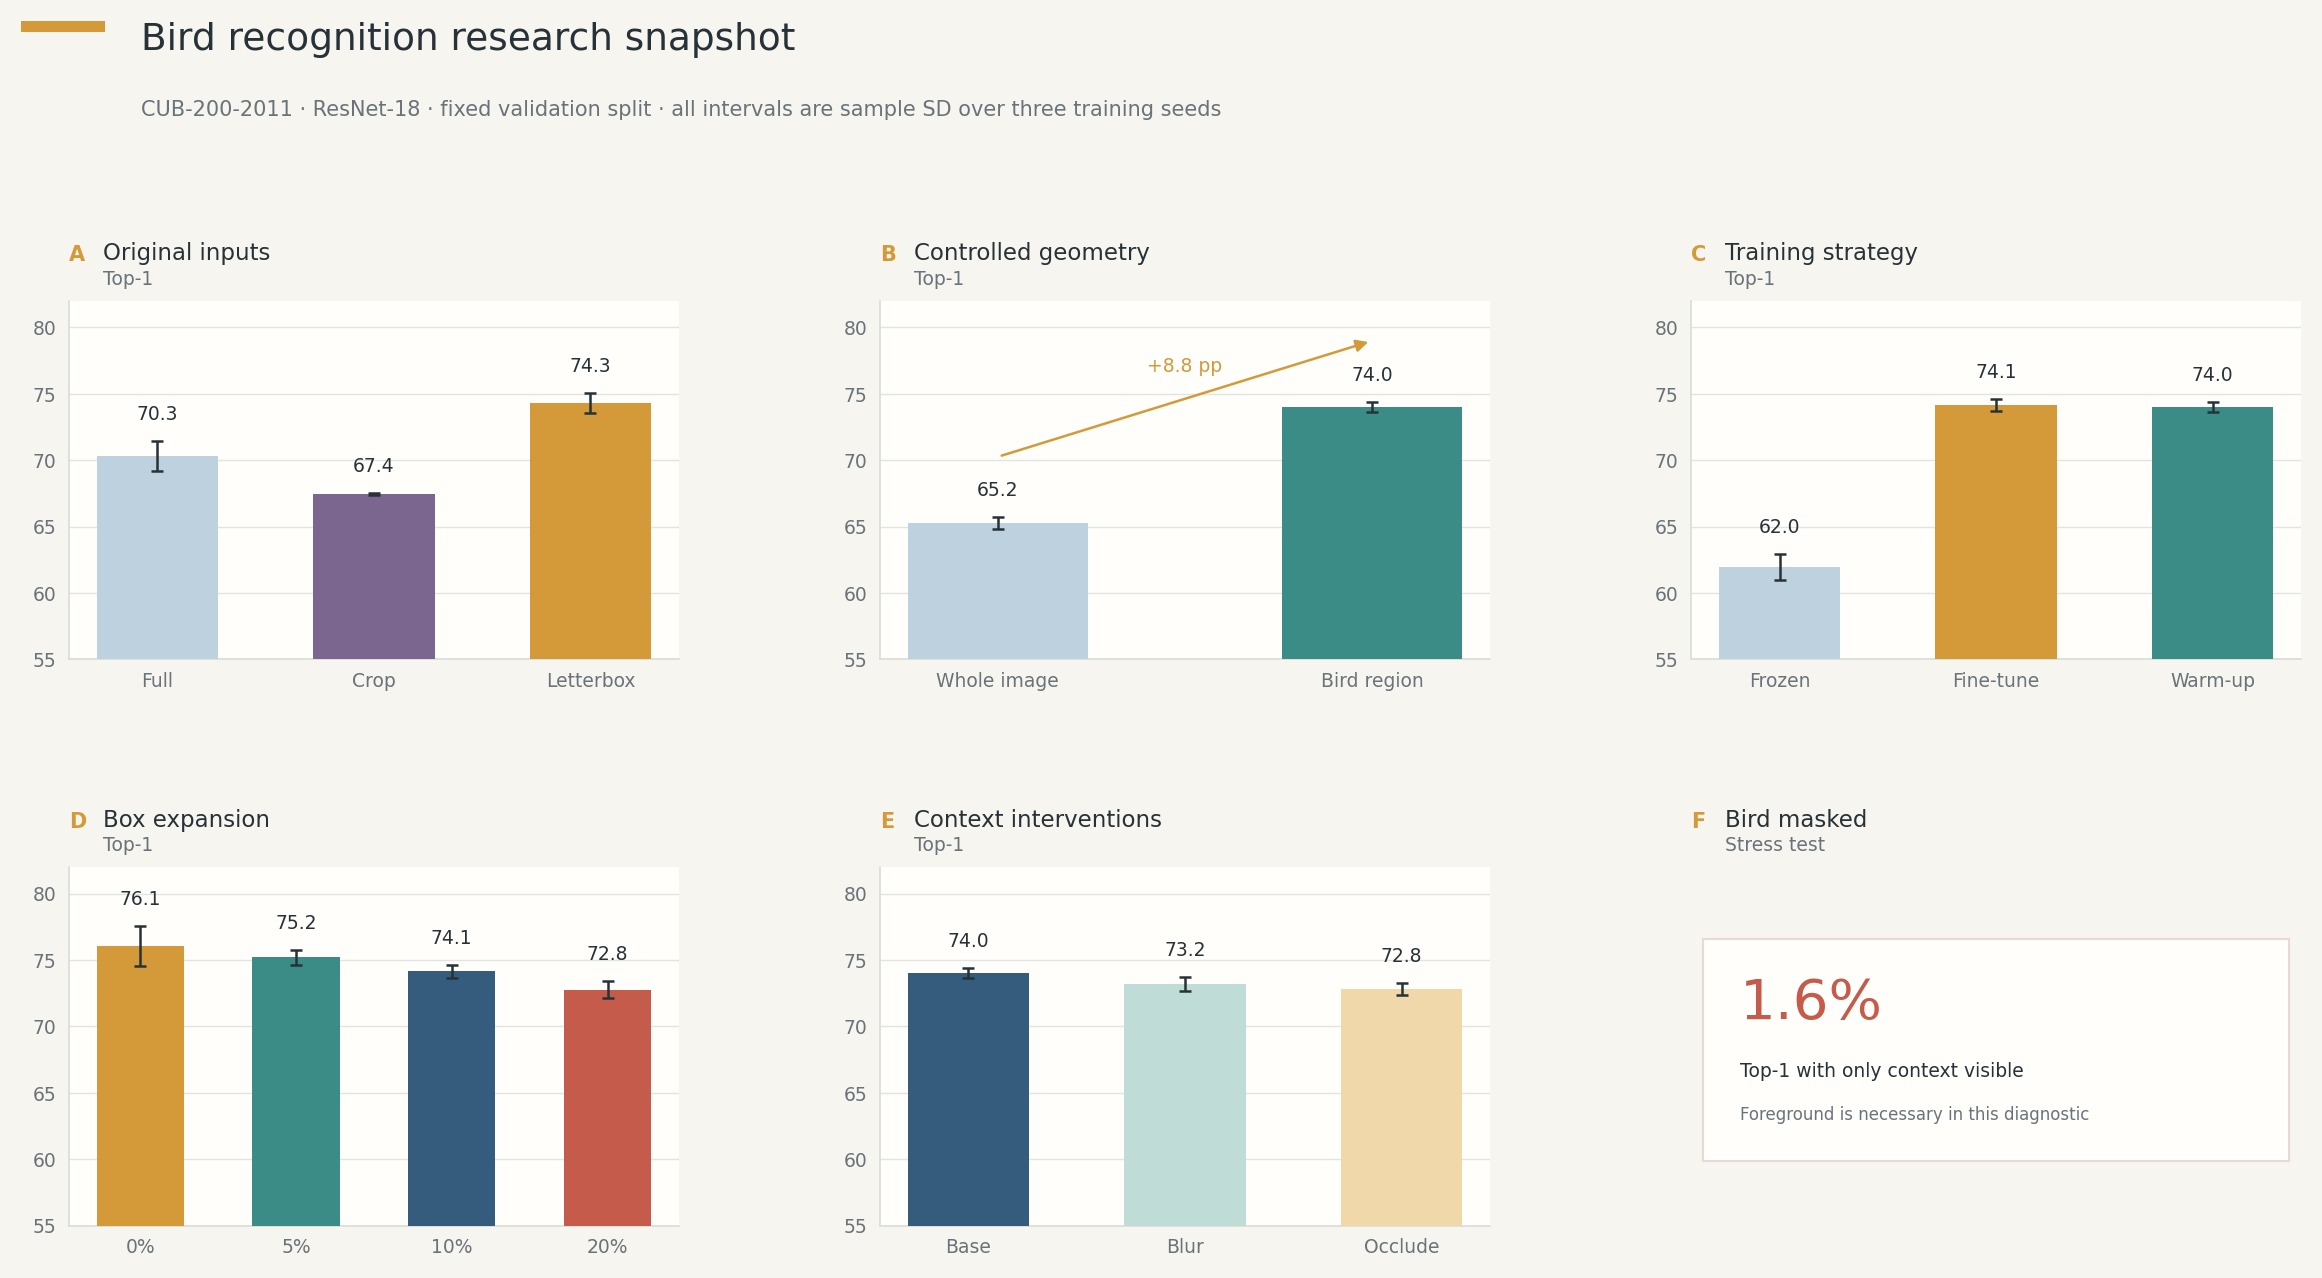
\includegraphics[width=0.96\textwidth]{images/research_overview.png}
\caption{Validation-only research overview. (A) Original input baseline.
(B) Matched whole-image versus bird-region letterboxing. (C) Frozen versus
fine-tuned training. (D) Box expansion ablation. (E) Context interventions.
(F) Bird-masked stress test. Error bars show sample standard deviation over
three training seeds.}
\label{fig:overview}
\end{figure*}

\section{Experiments}

\subsection{Original input comparison}

Table~\ref{tab:main-validation} summarizes the original three-way comparison.
Whole image reaches $70.31\%\pm1.13\%$ Top-1, center crop reaches
$67.44\%\pm0.05\%$, and bird letterbox reaches
$74.31\%\pm0.75\%$. Letterbox improves over the whole image by 4.00 points and
over center crop by 6.86 points, with the same direction under all three
seeds.

The center-crop result is informative: bird localization alone is not
sufficient. A narrow crop can remove context and can also clip a head, tail,
or other fine-grained evidence. Letterbox preserves the complete expanded
region and performs better.

\begin{table}[t]
\centering
\footnotesize
\setlength{\tabcolsep}{2pt}
\begin{tabular}{lccc}
\toprule
Validation condition & Top-1 & Top-5 & Macro-F1 \\
\midrule
Whole image & 70.31$\pm$1.13 & 91.42$\pm$0.22 & 70.02$\pm$0.92 \\
Center crop & 67.44$\pm$0.05 & 89.64$\pm$0.10 & 67.06$\pm$0.23 \\
Bird letterbox & \textbf{74.31$\pm$0.75} & \textbf{93.06$\pm$0.42} & \textbf{73.97$\pm$0.88} \\
\midrule
Whole + LB & 65.25$\pm$0.44 & 88.28$\pm$0.76 & 64.82$\pm$0.55 \\
Bird + LB & \textbf{74.00$\pm$0.36} & \textbf{93.44$\pm$0.42} & \textbf{73.91$\pm$0.33} \\
\midrule
Frozen backbone & 61.97$\pm$0.99 & 87.86$\pm$0.71 & 61.37$\pm$1.20 \\
Fine-tune E1 & \textbf{74.14$\pm$0.46} & 93.08$\pm$0.83 & \textbf{73.93$\pm$0.59} \\
Freeze 2, tune & 74.00$\pm$0.36 & \textbf{93.44$\pm$0.42} & 73.91$\pm$0.33 \\
\bottomrule
\end{tabular}
\caption{Validation results (\%; mean $\pm$ sample SD over seeds 42--44).
The lower two blocks are local controls and are not pooled with the original
three-way comparison.}
\label{tab:main-validation}
\end{table}

\subsection{Controlled geometry and training}

The matched whole-image and bird-region letterbox experiment produces
$65.25\%\pm0.44\%$ and $74.00\%\pm0.36\%$ Top-1, respectively. The paired
improvements are 9.33, 8.08, and 8.83 points for seeds 42, 43, and 44.
Because geometry and augmentation are held fixed, removal of random cropping
cannot by itself explain the gain. The crop still changes target scale and
retained context, so we avoid attributing the entire gain to background.

The training comparison shows a larger and more decisive effect. Frozen
features reach $61.97\%$ Top-1, while fine-tuning from epoch one reaches
$74.14\%$ and the two-epoch warm-up reaches $74.00\%$. Fine-tuning gains
$11.25$--$13.83$ points over the frozen backbone in every seed. Warm-up and
immediate fine-tuning differ by only 0.14 point on average, with inconsistent
seed-level signs. We therefore use immediate fine-tuning in the final
candidate; warm-up is not claimed to provide a stable benefit.

\subsection{Bird-box expansion ablation}

Figure~\ref{fig:margin} varies the box expansion while holding the network,
letterboxing, split, seeds, and ten-epoch fine-tuning budget fixed. Top-1 is
$76.06\%\pm1.54\%$ for margin 0\%, $75.19\%\pm0.54\%$ for 5\%,
$74.14\%\pm0.46\%$ for 10\%, and $72.78\%\pm0.63\%$ for 20\%.

Margins 0\% and 5\% both outperform 10\% under all three seeds, whereas 20\%
is worse under all three. The average 0\% minus 10\% difference is 1.92
points, and the 5\% minus 10\% difference is 1.06 points. The exact box has
the best mean, but its seed variation is larger; 5\% is the more stable
alternative. Margin 0\% and 5\% differ by only 0.86 point on average, and no
claim of statistical significance is made.

\begin{figure}[t]
\centering
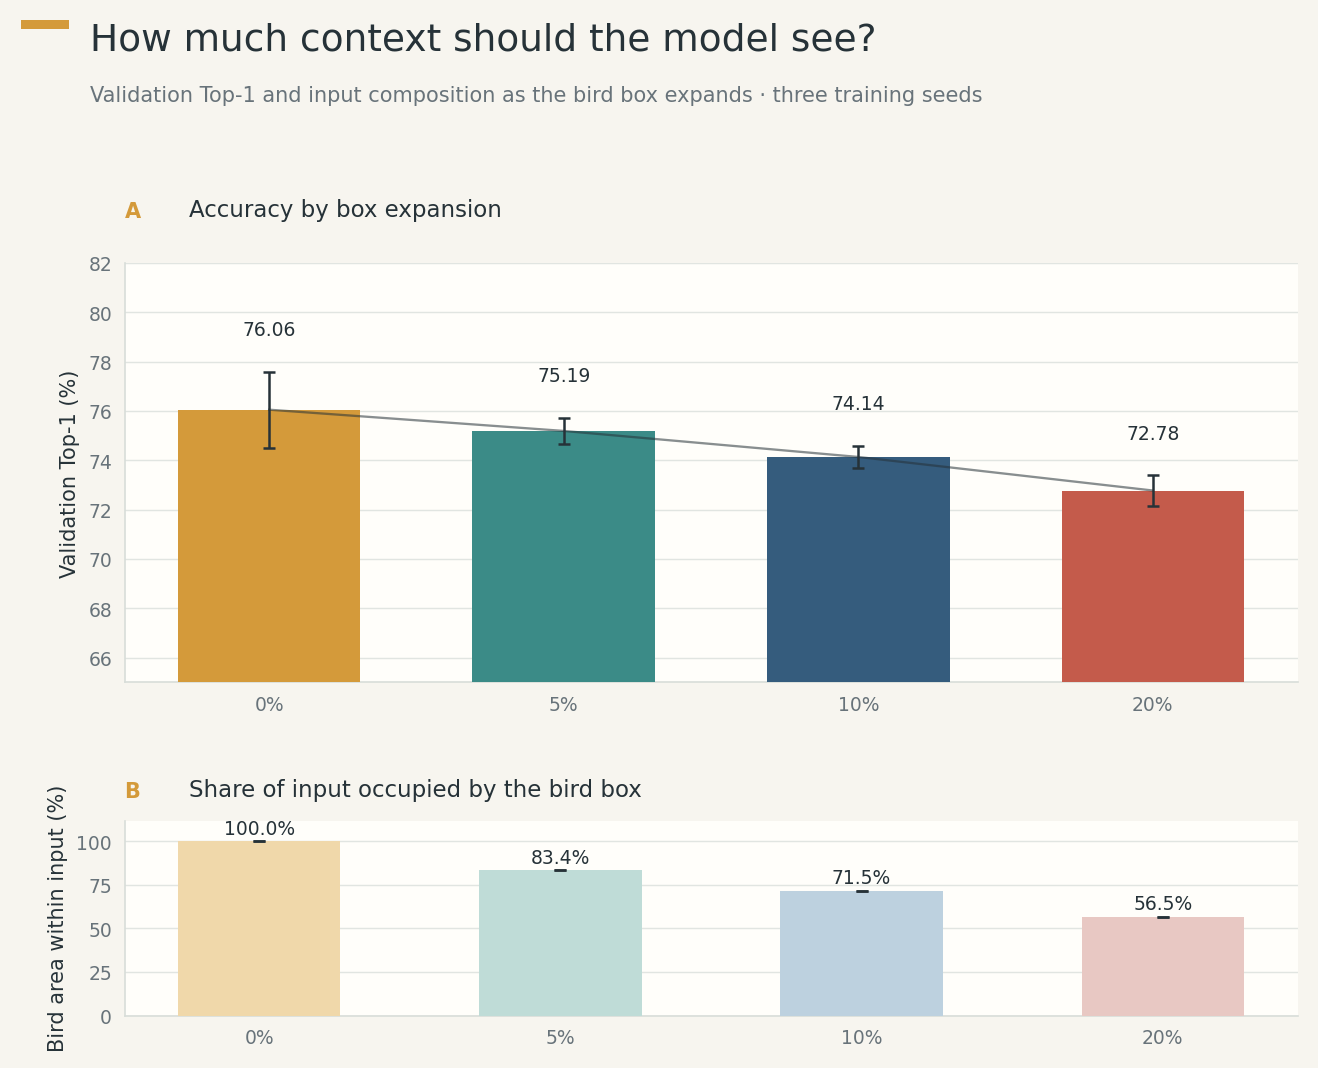
\includegraphics[width=\columnwidth]{images/margin_ablation.png}
\caption{Bird-box expansion ablation. The lower panel reports the mean fraction
of the network input occupied by the bird box. Increasing the margin changes
target scale, context area, padding, and effective pixels simultaneously.}
\label{fig:margin}
\end{figure}

\section{Background Analysis and Interpretation}

\subsection{Interventions inside the 10\% view}

We use the three 10\%-expanded letterbox models for a validation-only stress
test. The baseline result is $74.00\%$ Top-1. Gaussian blur of context outside
the tight box changes Top-1 to $73.19\%$; replacing context with a neutral
color changes it to $72.83\%$. Both directions are consistent across seeds,
but the degradation is below 1.2 points. A bird-masked condition that keeps
only context collapses to $1.61\%$ Top-1.

Figure~\ref{fig:background-size} shows the same pattern across bird-size
groups: context perturbations have limited effect, while masking the bird
causes near-complete failure. The smallest group contains only 33 validation
images and is exploratory. The evidence supports foreground dependence in
normal prediction, but the bird-masked test is a distribution shift and does
not prove that background has no role.

\begin{figure*}[t]
\centering
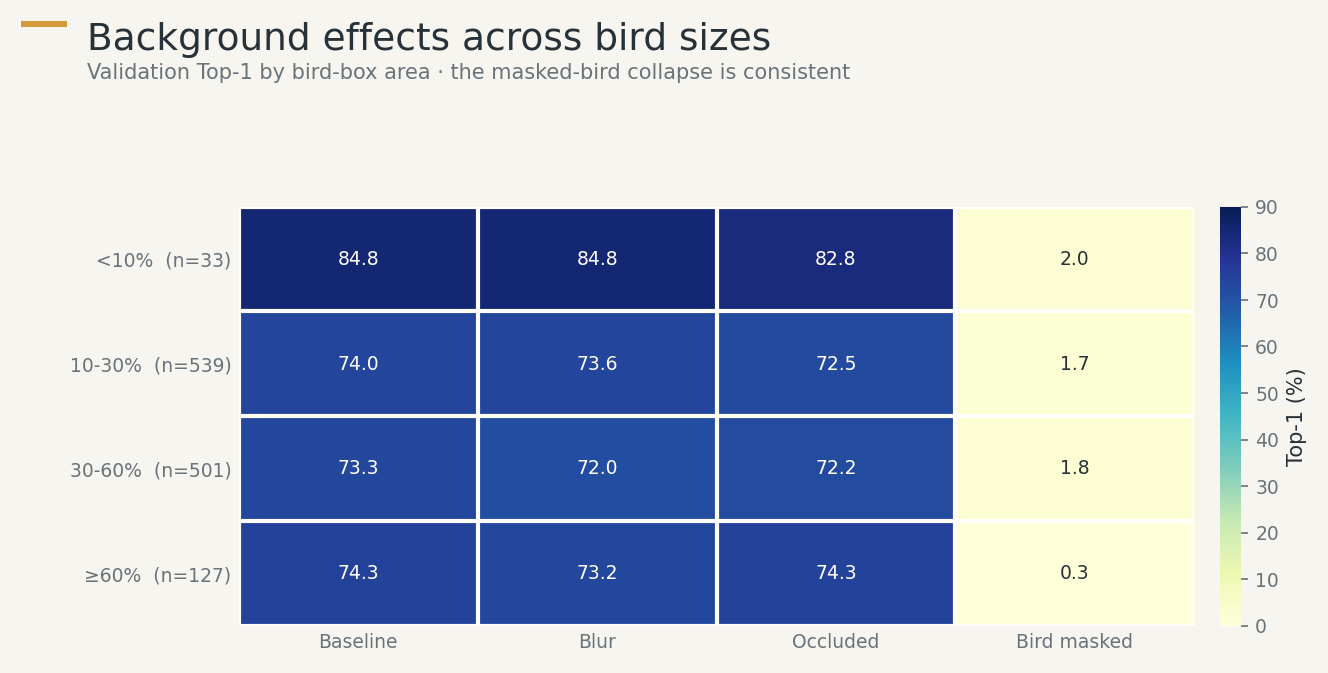
\includegraphics[width=0.88\textwidth]{images/background_by_bird_size.png}
\caption{Validation Top-1 by bird-box area under four context conditions.
Context blur and occlusion cause small changes; masking the bird causes a
large failure in every size group.}
\label{fig:background-size}
\end{figure*}

\subsection{Grad-CAM}

Figure~\ref{fig:gradcam} shows representative correct predictions and
high-confidence failures for the selected seed-43 model. Correct examples
typically place attention on the bird's head, bill, torso, or wing patterns.
Failures can place attention on broad body regions or surrounding structure
without isolating the cue needed to separate similar species. The selected
cases are explanatory rather than a random sample, and Grad-CAM is only a
coarse visualization.

\begin{figure*}[t]
\centering
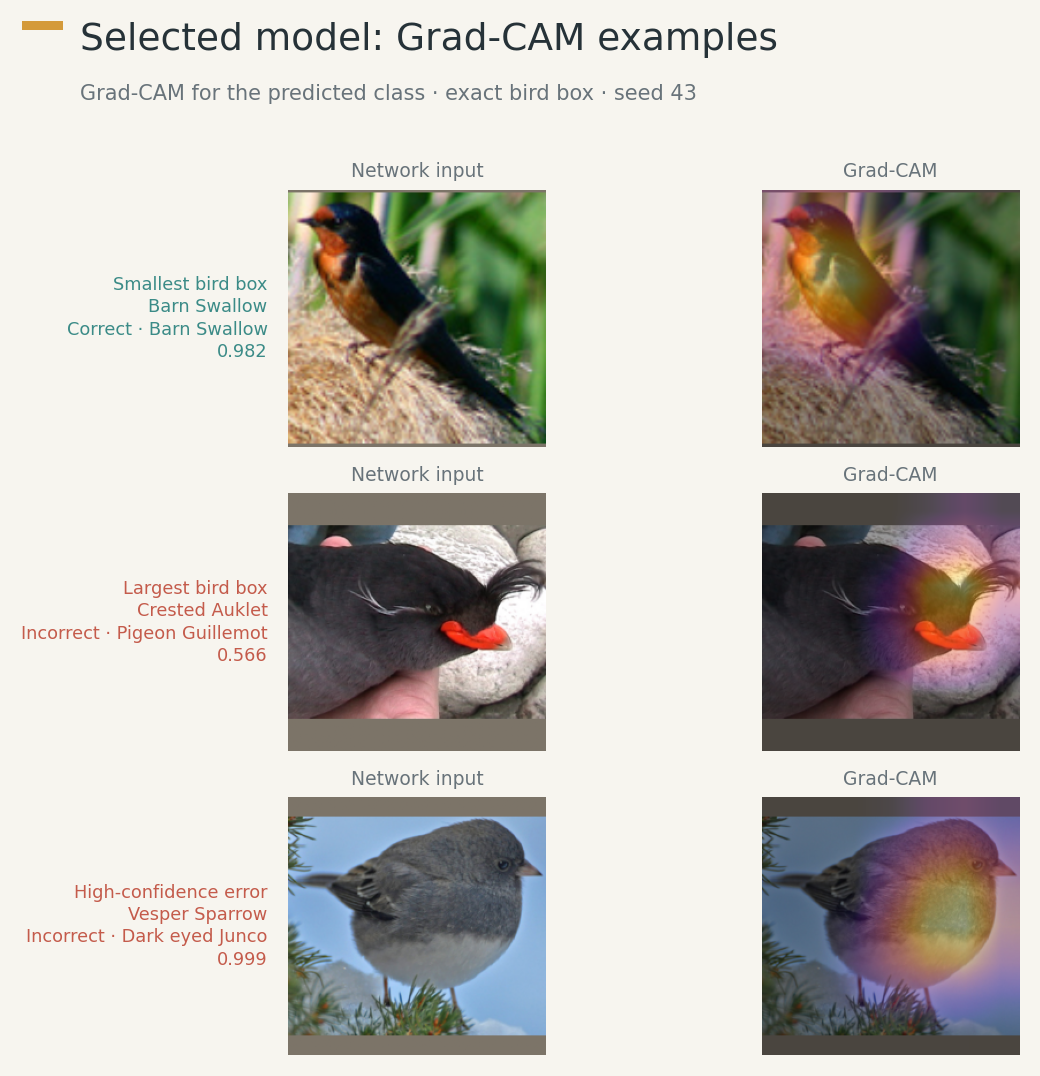
\includegraphics[width=0.64\textwidth]{images/gradcam_compact.png}
\caption{Grad-CAM for the selected margin-0\% model. A smallest-box success,
largest-box failure, and high-confidence failure illustrate head/body
attention and important failure modes.}
\label{fig:gradcam}
\end{figure*}

\section{Final Frozen Model and Test Evaluation}

The final model was selected using validation evidence only: margin 0\%
achieved the best mean, and seed 43 was the best checkpoint within that
condition. The model, preprocessing, split, and checkpoint were copied into a
frozen directory before the official test partition was opened.

Table~\ref{tab:test} reports the single post-freeze evaluation. Top-1 is
$77.87\%$, Top-5 is $94.15\%$, and Macro-F1 is $77.85\%$ on 5,794 images.
The validation Top-1 of the same checkpoint is $77.83\%$. The 0.04-point test
difference is small and descriptive; no significance test is inferred.
No checkpoint, seed, margin, or hyperparameter was changed after observing
the test results.

\begin{table}[t]
\centering
\small
\begin{tabular}{lccc}
\toprule
Partition & Top-1 & Top-5 & Macro-F1 \\
\midrule
Validation (1,200) & 77.83 & 93.42 & 77.63 \\
Official test (5,794) & \textbf{77.87} & \textbf{94.15} & \textbf{77.85} \\
\bottomrule
\end{tabular}
\caption{Frozen-model results (\%). Model selection used validation only.}
\label{tab:test}
\end{table}

Figure~\ref{fig:test} compares validation and test metrics. The consistency
between partitions suggests that the validation protocol was reasonably
representative. Per-class test accuracy has median 83.33\% and ranges from
23.33\% to 100\%, showing that aggregate accuracy hides difficult species.

\begin{figure}[t]
\centering
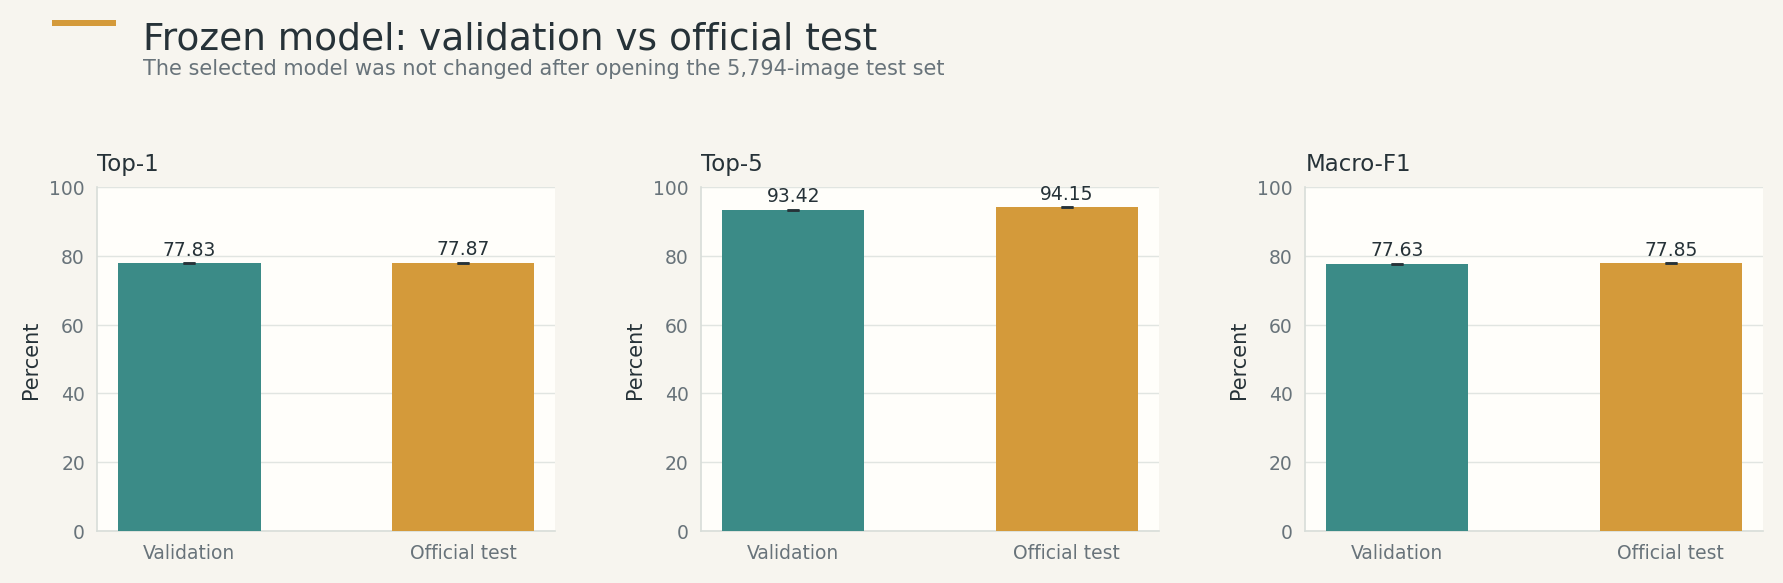
\includegraphics[width=\columnwidth]{images/validation_vs_test.png}
\caption{Selected frozen model on validation and the single official test
evaluation. The model was not modified after test evaluation.}
\label{fig:test}
\end{figure}

Figure~\ref{fig:confusions} shows the most frequent official-test confusion
pairs. Many errors link visually similar species: shrikes, crows and ravens,
terns, flycatchers, nightjars, and hummingbirds. These are plausible
fine-grained confusions rather than random label failures.

\begin{figure}[t]
\centering
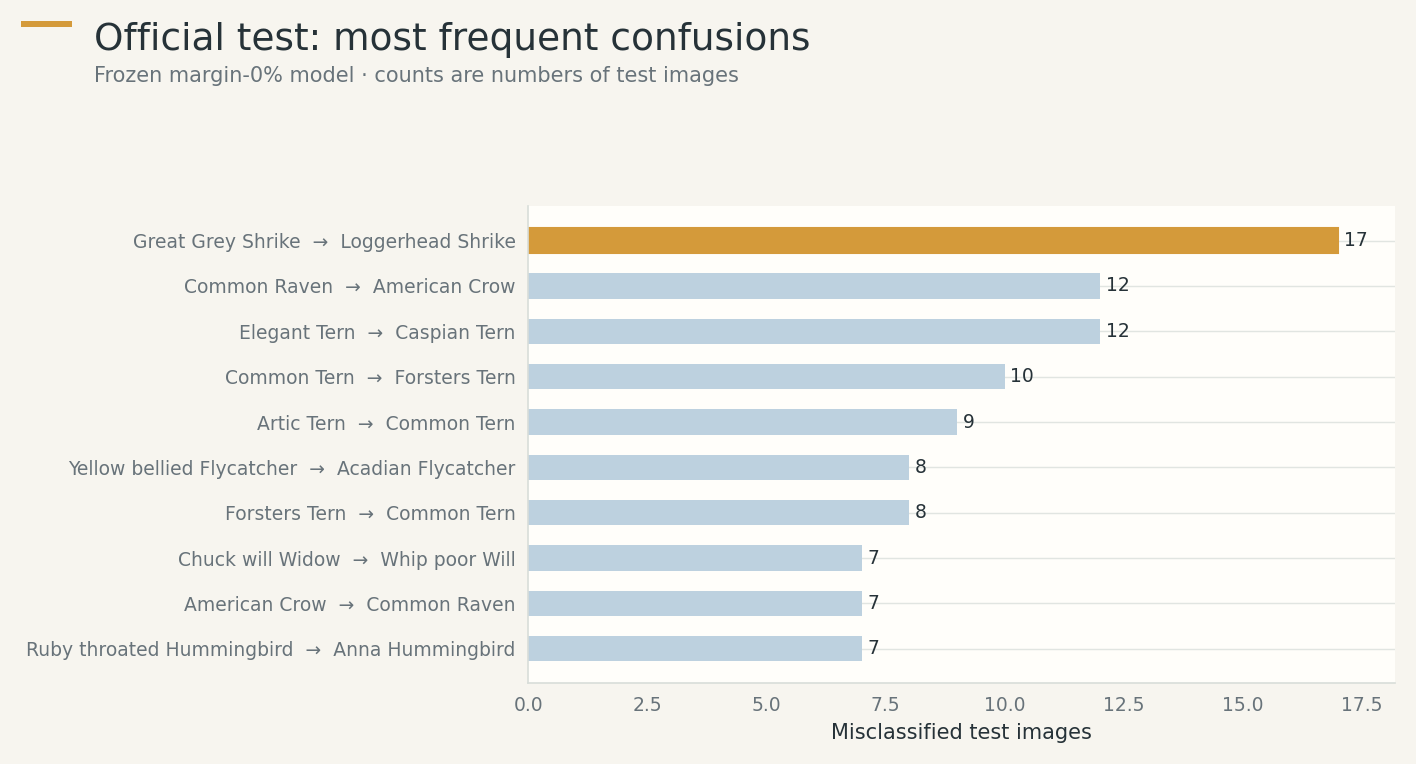
\includegraphics[width=\columnwidth]{images/top_confusion_pairs.png}
\caption{Most frequent official-test confusion pairs for the frozen model.}
\label{fig:confusions}
\end{figure}

\section{Discussion and Limitations}

The main empirical result is that both foreground localization and backbone
fine-tuning are necessary in this project. Frozen features perform poorly
despite a strong ImageNet initialization. Bird-region inputs outperform
whole-image inputs under matched geometry, and tighter boxes outperform larger
context windows. The background-only stress test strongly suppresses
recognition, while context blur and occlusion have small aggregate effects.
Together, these results support a foreground-centered interpretation.

The evidence nevertheless has important limits. First, all bird-aware methods
use ground-truth CUB boxes. The selected system is not an automatic detector
and requires a box at inference. Second, changing the margin simultaneously
changes target scale, context, padding, and effective pixels; it is not a pure
background manipulation. Third, context perturbations are inference-time
distribution shifts rather than retraining experiments. Fourth, CUB may overlap
with ImageNet, so pretraining exposure is a shared confound across all
conditions. Fifth, only ResNet-18 is tested, and three seeds provide
stability evidence rather than a general claim. Finally, probabilities are
not calibrated, and Grad-CAM is not a strict causal method.

The 77.87\% test Top-1 is a result for a 200-class benchmark with exact
localization annotations, not an unconstrained wild-bird identification
system. A practical deployment would need either manual boxes or an
independent detector, and its errors should be evaluated under that full
pipeline.

\section{Conclusion}

We presented a controlled study of foreground and input geometry for
fine-grained bird recognition. Exact bird boxes with aspect-ratio-preserving
letterboxing outperform whole-image and center-crop baselines; the gain
persists under matched geometry; and full fine-tuning is substantially better
than frozen features. The selected model reaches 77.87\% Top-1 and 77.85\%
Macro-F1 on the official test set. Background perturbations inside the
bird-centered view cause only small changes, whereas masking the bird causes
near-complete failure. Future work should compare automatic detection plus
recognition, test additional backbones and augmentation policies, calibrate
uncertainty, and evaluate whether the same conclusions hold on bird images
outside CUB.

\section*{Implementation and AI Disclosure}
The implementation, experiment orchestration, and figure-generation code were
developed with iterative assistance from Codex. The authors reviewed the data
splits, training protocol, evaluation logic, metric calculations, and reported
limitations. Public datasets, pretrained weights, libraries, and prior work
are cited in the references.

\begin{thebibliography}{9}
\small
\bibitem{wah2011cub}
C. Wah, S. Branson, P. Welinder, P. Perona, and S. Belongie.
\newblock The Caltech-UCSD Birds-200-2011 Dataset.
\newblock \emph{CNS-TR-2011-001}, 2011.

\bibitem{he2016resnet}
K. He, X. Zhang, S. Ren, and J. Sun.
\newblock Deep Residual Learning for Image Recognition.
\newblock In \emph{CVPR}, 2016.

\bibitem{deng2009imagenet}
J. Deng, W. Dong, R. Socher, L.-J. Li, K. Li, and L. Fei-Fei.
\newblock ImageNet: A Large-Scale Hierarchical Image Database.
\newblock In \emph{CVPR}, 2009.

\bibitem{selvaraju2017gradcam}
R. R. Selvaraju, M. Cogswell, A. Das, R. Vedantam, D. Parikh, and D. Batra.
\newblock Grad-CAM: Visual Explanations from Deep Networks via
Gradient-Based Localization.
\newblock In \emph{ICCV}, 2017.

\bibitem{pytorch2019transfer}
PyTorch.
\newblock Transfer Learning for Computer Vision Tutorial.
\newblock \url{https://docs.pytorch.org/tutorials/beginner/transfer_learning_tutorial.html}
\end{thebibliography}

\end{document}
